\documentclass[12pt]{../packages/thesis}  %12pt is larger than 11pt

\usepackage{titlesec}
   \titleformat{\chapter}
      {\normalfont\large}{Chapter \thechapter:}{1em}{}

      \usepackage[pdftex]{graphicx}
\usepackage{float}
\usepackage{mathrsfs,amsmath}
\numberwithin{equation}{chapter}
\setcounter{secnumdepth}{4}
\titleformat{\paragraph}
{\normalfont\normalsize\bfseries}{\theparagraph}{1em}{}
\titlespacing*{\paragraph}
{0pt}{3.25ex plus 1ex minus .2ex}{1.5ex plus .2ex}
\usepackage{chngcntr}
\counterwithin{table}{chapter}
\counterwithin{figure}{chapter}
\usepackage{cite}
\usepackage{lscape}
\usepackage{indentfirst}
\usepackage{latexsym}
\usepackage{multirow}
\usepackage{tabls}
\usepackage{wrapfig}
\usepackage{../packages/slashbox}
\usepackage{longtable}
\usepackage{supertabular}
\usepackage{subfigure}


\newcommand{\tbsp}{\rule{0pt}{18pt}} %used to get a vertical distance after \hline
\renewcommand{\baselinestretch}{2}
\setlength{\textwidth}{5.9in}
\setlength{\textheight}{9in}
\setlength{\topmargin}{-.50in}
%\setlength{\topmargin}{0in}    %use this setting if the printer makes the the top margin 1/2 inch instead of 1 inch
\setlength{\oddsidemargin}{.55in}
\setlength{\parindent}{.4in}
\pagestyle{empty}

\begin{document}

\pagenumbering{arabic}
\setcounter{page}{1}


\chapter{Saddle Point Method}\label{appendix_saddle_point_method}
A contour integral representation of the Bessel function in the complex $z$-plane is \cite{arfken_weber}, \cite{nist_handbook}:

\begin{equation}
  J_{\nu}(x) = \frac{1}{j2\pi}\int\limits_{\mathcal{C}}e^{\frac{1}{2}x\left(z- \frac{1}{z} \right)} \frac{dz}{z^{\nu+1}}
  \label{sp_eq:1}
\end{equation}
\renewcommand{\baselinestretch}{2} \small\normalsize

The integrand is multi-valued when $\nu$ is not an integer, so we can define a branch cut along the real axis and the overall contour, $\mathcal{C}$, as shown in Figure \ref{sp_fig:1}.

\begin{figure}[H]
  \begin{center}
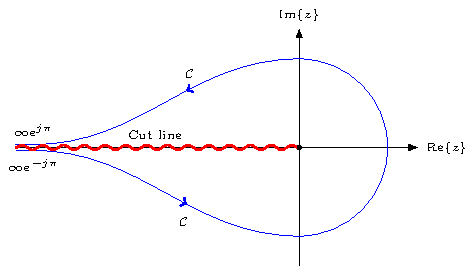
\includegraphics[width=5in]{../media/hankel_contours-figure0.pdf}
  \end{center}
  \renewcommand{\baselinestretch}{1} \small\normalsize
  \begin{quote}
    \caption[Complex Contour for Bessel Function]{ Complex Contour for Bessel Function\label{sp_fig:1}}
  \end{quote}
\end{figure}
\renewcommand{\baselinestretch}{2} \small\normalsize

We can deform the contour, $\mathcal{C}$, so that it goes to the origin and then split it into two parts, an upper contour ($\mathcal{C}_1$) and a lower contour ($\mathcal{C}_2$). Integration along the upper contour represents the Hankel function of the first kind, while integration along the lower contour represents the Hankel function of the first kind. The resulting contour is shown in Figure \ref{sp_fig:2}.

\begin{figure}[H]
  \begin{center}
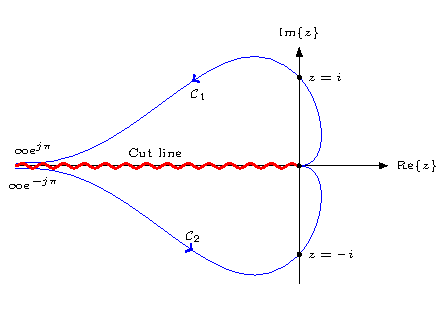
\includegraphics[width=5in]{../media/hankel_contours-figure1.pdf}
\end{center}
  \renewcommand{\baselinestretch}{1}\small\normalsize
  \begin{quote}
    \caption[Complex Contour for Hankel Functions]{Complex Contour for Hankel Functions\label{sp_fig:2}}
  \end{quote}
\end{figure}
\renewcommand{\baselinestretch}{2} \small\normalsize

The integral representations of the Hankel functions are then:
\begin{equation}
  \begin{gathered}
    H_{\nu}^{(1)}(x) = \frac{1}{j\pi}\int\limits_{\mathcal{C}_1}e^{\frac{1}{2}x\left(z- \frac{1}{z} \right)} \frac{dz}{z^{\nu+1}} \\
    H_{\nu}^{(2)}(x) = \frac{1}{j\pi}\int\limits_{\mathcal{C}_2}e^{\frac{1}{2}x\left(z- \frac{1}{z} \right)} \frac{dz}{z^{\nu+1}} 
    \end{gathered}
  \label{sp_eq:2}
  \end{equation}
\renewcommand{\baselinestretch}{2} \small\normalsize

We can find an asymptotic solution of the Hankel functions through the saddle point method, which applies to integrals in the form of $I = \int\limits_{\mathcal{C}}g(z)e^{xh(z)}dz$. We will work with the Hankel function of the second kind, $H_{\nu}^{(2)}$, as that represents a forward traveling wave.

The general idea of the saddle point method is expand the exponential term, $h(z)$ in a Taylor series about the saddle point so that the first derivative of $h$ goes to zero. We will use the phase of $h$ to ensure the dominant contribution to the integral comes from the saddle point. In Equation \ref{sp_eq:2}, $h = \frac{1}{2}\left(z-\frac{1}{z}\right)$, so the first derivative is $\frac{dh}{dz} = \frac{1}{2}\left(1+\frac{1}{z^2}\right)$, and the second derivative is $\frac{d^2h}{dz^2} = -\frac{1}{z^3}$. From the first derivative, $h$ has a saddle point ($\frac{dh}{dz}=0$) at $z=\pm j$. Along contour $\mathcal{C}_2$, the only saddle point is $z=-j$, so that is the one we will use.

The Taylor expansion of $h$ is then:

\begin{equation}
  \begin{gathered}
    h(z) \approx h\bigg|_{z=-j} + \frac{1}{2}\frac{d^2h}{dz^2}\bigg|_{z=-j}\left(z+j \right)^2\\
    h(z) \approx -j + \frac{j}{2}\left(z+j \right)^2 
    \end{gathered}
  \label{sp_eq:3}
  \end{equation}
\renewcommand{\baselinestretch}{2} \small\normalsize

Substituting this approximation for $h$ into Equation \ref{sp_eq:2} and remembering that $g(z) \rightarrow g(z)|_{z=-j}$ yields:

\begin{equation}
  \begin{gathered}
    H_{\nu}^{(2)}(x) \approx \frac{1}{j\pi}\int\limits_{\mathcal{C}_2}e^{x\left[-j + \frac{j}{2}\left(z+j \right)^2 \right]} \frac{dz}{(-j)^{\nu+1}} \\
    H_{\nu}^{(2)}(x) \approx \frac{1}{j\pi}e^{-jx}\int\limits_{\mathcal{C}_2}e^{x\frac{j}{2}\left(z+j \right)^2}(-j)^{-\nu - 1} dz \\
    H_{\nu}^{(2)}(x) \approx \frac{1}{\pi}e^{-jx}e^{-j\frac{\pi}{2}}e^{-j\frac{3\pi}{2}\left(\nu +1\right)}\int\limits_{\mathcal{C}_2}e^{x\frac{j}{2}\left(z+j \right)^2} dz \\
    H_{\nu}^{(2)}(x) \approx \frac{1}{\pi}e^{-j\left[x +\frac{\pi}{2} +\frac{3\pi}{2} + \nu\frac{3\pi}{2}\right]}\int\limits_{\mathcal{C}_2}e^{x\frac{j}{2}\left(z+j \right)^2} dz \\
     H_{\nu}^{(2)}(x) \approx \frac{1}{\pi}e^{-j\left[x - \nu\frac{\pi}{2}\right]}\int\limits_{\mathcal{C}_2}e^{x\frac{j}{2}\left(z+j \right)^2} dz 
    \end{gathered}
  \label{sp_eq:4}
  \end{equation}
\renewcommand{\baselinestretch}{2} \small\normalsize

We need to ensure that we approach the saddle point along the path of steepest descent, where the path $\mathcal{C}_2$ travels from $\infty$ to $0$ with $z$ having negative phase. By inspection we can see that the condition $\left(z+j \right)^2 \rightarrow j$ forces the integral to go to zero for large $x$. We can write this condition more explicitly in terms of phase as:

\begin{equation}
  \begin{gathered}
    \left(z + j \right)^2=j \\
    r^2e^{j2\theta} = e^{j\frac{\pi}{2}} \\
    \theta = \frac{\pi}{4}
    \end{gathered}
  \label{sp_eq:5}
  \end{equation}
\renewcommand{\baselinestretch}{2} \small\normalsize

Equation \ref{sp_eq:5} tells us that the path of integration must enter the saddle point ($z=-j$) with a phase angle of $\frac{\pi}{4}$ radians. We can use a substitution of variables, $t=(z+j)e^{j\frac{\pi}{4}}$, so that $dt = dze^{j\frac{\pi}{4}}$:

\begin{equation}
  \begin{gathered}
    H_{\nu}^{(2)}(x) \approx \frac{1}{\pi}e^{-j\left[x - \nu\frac{\pi}{2}\right]}\int\limits_{\mathcal{C}_2}e^{x\frac{j}{2}t^2e^{j\frac{\pi}{2}}} dte^{j\frac{\pi}{4}} \\
    H_{\nu}^{(2)}(x) \approx \frac{1}{\pi}e^{-j\left[x - \nu\frac{\pi}{2}\right]}e^{j\frac{\pi}{4}}\int\limits_{\mathcal{C}_2}e^{-\frac{xt^2}{2}} dt \\
     H_{\nu}^{(2)}(x) \approx  \frac{1}{\pi}e^{-j\left[x - \nu\frac{\pi}{2} - \frac{\pi}{4}\right]}\int\limits_{-\infty}^{\infty}e^{-\frac{xt^2}{2}} dt \\
    H_{\nu}^{(2)}(x) \approx \frac{1}{\pi}e^{-j\left[x - \nu\frac{\pi}{2} - \frac{\pi}{4}\right]}\sqrt{\frac{2\pi}{x}}\\
    \end{gathered}
  \label{sp_eq:6}
  \end{equation}
\renewcommand{\baselinestretch}{2} \small\normalsize

\noindent A final simplification yields the asymptotic form of the Hankel function:
\begin{equation}
    \boxed{H_{\nu}^{(2)}(x) \approx \sqrt{\frac{2}{\pi x}}e^{-j\left[x - \nu\frac{\pi}{2} - \frac{\pi}{4}\right]}}
  \label{sp_eq:7}
  \end{equation}
\renewcommand{\baselinestretch}{2} \small\normalsize

Figure \ref{sp_fig:3} shows a comparison between the real and imaginary components of the analytic and asymptotic forms of the Hankel function, $H_0^{(2)}$, and demonstrates that the asymptotic form is valid for large $x$.

\begin{figure}[H]
  \begin{center}
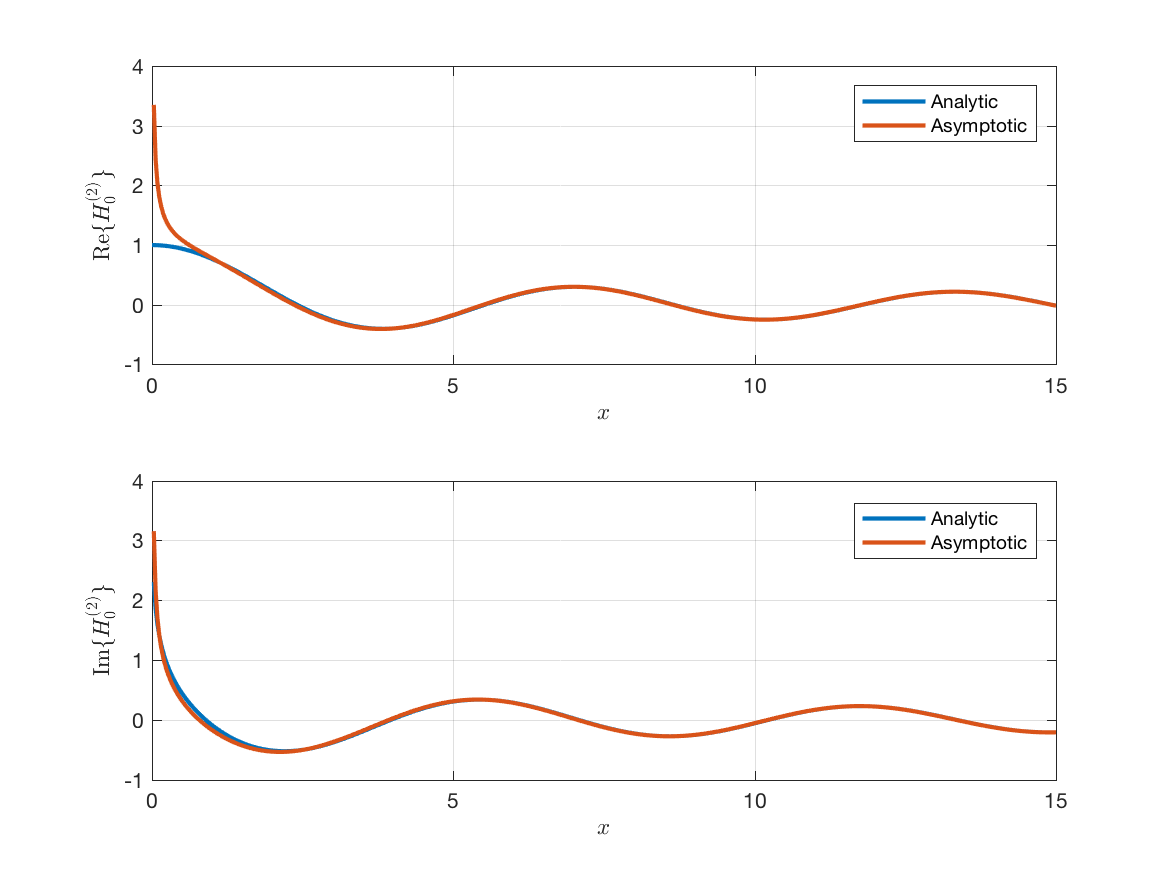
\includegraphics[width=5in]{../media/hankel_error.png}
\end{center}
  \renewcommand{\baselinestretch}{1}\small\normalsize
  \begin{quote}
    \caption[Analytic vs. Asymptotic Forms of Hankel Function]{Analytic vs. Asymptotic Forms of Hankel Function\label{sp_fig:3}}
  \end{quote}
\end{figure}
\renewcommand{\baselinestretch}{2} \small\normalsize


\newpage
\bibliographystyle{unsrt} 
\bibliography{background_bib}

\end{document}
